
\iffalse{
	\subsection{Notation}
	For vectors $x,y\in \mathbb{R}_{n}$ we say $x$ dominates $y$ if $x_i\geq y_i$ for $i= 1,\ldots,n$. For $m\times n$ matrix $A$, let $A_j$ be the $j$-th row of $A$ and $A^j$ be the $j$-th column of $A$. For a set $S$ of vectors in $\mathbb{R}_{n}$, $\conv(S)$ is the convex hull of all the points in $S$.
}\fi
\section{Finding a Feasible Solution}\label{sec:domTOIP}
In this section we give the algorithm for DomToIP and prove its performance (Theorem~\ref{domtoIP}).

Consider an instance $I=(A,b)$ of the IP formulation. Define sets $S(I)$ and $P(I)$ as in (\ref{S}) and (\ref{P}), respectively. Assume $S(I)\subseteq \{0,1\}^n$ and $P(I)\subseteq [0,1]^n$. For simplicity in the notation we assume an instance $I$ and denote $P(I),S(I),$ and $g(I)$ by $P$, $S$, and $g$ for this section and the next section. Also, for both sections let $x^*$ be the optimal solution to the LP formulation and assume $t=|\spp(x^*)|$. Without loss of generality we can assume $x^*_i = 0$ for $i=t+1,\ldots,n$.
\cindy{TODO: Is this something that should be clear to the reader with what they know at this point? Does it need an explanation? Does it need an explanation at the end of this section or the next?}\arash{this is just a relabeling of the indices.} \cindy{Sorry.  I didn't understand that you meant the solution has that property. Right? The vector $x$ isn't defined in this paragraph and it's not in the next lemma either. If $x$ is the output of DomToIP, then we should say that.  ``Without loss of generality the solution $x$ returned by DomToIP has ...''}\arash{I see your point, please see if the change made it better}

In this section we prove Theorem \ref{domtoIP}. In fact, we prove a stronger result. 
\begin{lemma}\label{domlemma}
	Given $\tilde{x}\in \dom(P)$ and $\tilde{x}\in \{0,1\}^n$, there is an algorithm (the DomToIP algorithm) that finds $\bar{x}\in S$ in polynomial time, such that $\bar{x}\leq \tilde{x}$.\end{lemma}
Notice that Lemma \ref{domlemma} implies Theorem \ref{domtoIP}, since it is easy to obtain an integer point in $\dom(P)$: numerically rounding up $x^*$ (or any fractional point in $P$) gives us a point in $\dom(P)$. Hence, we can assume in the proof below that $\tilde{x}_i= 0$ for $i=t+1,\ldots,n$. 
\arash{I also made a change based on the change above}
\subsection{Proof of Lemma \ref{domlemma}: The DomToIP Algorithm}

We start by introducing an algorithm that ``fixes" the variables iteratively, starting from the first coordinate and ending at the $t$-th coordinate. Suppose we run the algorithm for $\ell\in \{0,\ldots,t-1\}$ iterations and in each iteration we find $x^{(\ell)}\in \dom(P)$  such that $x^{(\ell)}_i\in \{0,1\}$ for $i=1,\ldots,\ell$. Notice that we can set $x^{(0)}=\tilde{x}$. Now consider the following linear program. The variables of this linear program are the $z\in \mathbb{R}^n$ variables.
\begin{align}
\DOMtoS(x^{(\ell)})\quad\quad& \min\quad \;z_{\ell+1}\\
&\;\text{s.t.} \quad \;\;Az\geq b \\
&\;{\color{white}{\text{s.t.}} }\quad \;\; \; z_j = x^{(\ell)}_j \quad \; j =1,\ldots, \ell\\
&\;{\color{white}{\text{s.t.}} }\quad \; \;\; z_j \leq x^{(\ell)}_j \quad \; j = \ell+1,\ldots,n\\
&\;{\color{white}{\text{s.t.}} }\quad \; \;\; z\;\geq 0
\end{align}

If the optimal value to $\DOMtoS(x^{(\ell)})$ is 0, then let $x^{(\ell+1)}_{\ell+1} = 0$. Otherwise if the optimal value is strictly positive let $x^{(\ell+1)}_{\ell+1} = 1$. Let $x^{(\ell+1)}_j = x^{(\ell)}_j$ for $j\in [n]\setminus \{\ell+1\}$ (See Algorithm \ref{domtoIPalg}).

The above procedure suggests how to find $x^{(\ell+1)}$ from $x^{(\ell)}$. The DomToIP algorithm initializes with $x^{(0)}=\tilde{x}$ and  iteratively calls this procedure in order to obtain $x^{(t)}$. 

\vspace*{10pt}
\begin{algorithm}[h]
	\KwIn{$\tilde{x}\in \dom(P)$, $\tilde{x}\in \{0,1\}^n$ }
	\KwOut{$x^{(t)} \in S$, $x^{(t)}\leq \tilde{x}$}
	$x^{(0)}\leftarrow \tilde{x}$\\
	\For{$\ell = 0$ \textbf{to} $t-1$}{
		$x^{(\ell+1)} \leftarrow x^{(\ell)}$\\
		$\eta \leftarrow$ optimal value of $ \DOMtoS(x^{(\ell)})$\\
		\eIf{$\eta = 0$}{
			$x^{(\ell+1)}_{\ell+1} \leftarrow 0$\
		}{
			$x^{(\ell+1)}_{\ell+1} \leftarrow 1$
		}
	}
	\caption{The DomToIP algorithm}
	\label{domtoIPalg}
\end{algorithm}
\vspace*{10pt}

We prove that indeed $x^{(t)}\in S$. First, we need to show that in any iteration $\ell=  0,\ldots,t-1$ of DomToIP that $\DOMtoS(x^{(\ell)})$ is feasible. We show something stronger. For $\ell=0,\ldots,t-1$ let
\begin{align*}
\LP^{(\ell)}&= \{z\in P\; : \; z\leq x^{(\ell)} \mbox{ and } z_j=x_j^{(\ell)} \mbox{ for } j\in [\ell]\}, \text{ and}\\
\IP^{(\ell)}&= \{z\in \LP^{(\ell)}\; : \; z\in \{0,1\}^n\}.
\end{align*}
Notice that if $\LP^{(\ell)}$ is a non-empty set then $\DOMtoS(x^{(\ell)})$ is feasible. We show by induction on $\ell$ that $\LP^{(\ell)}$ and $\IP^{(\ell)}$ are not empty sets for $\ell=0,\ldots,t-1$. First notice that $\LP^{(0)}$ is clearly feasible since by definition $x^{(0)}\in \dom(P)$, meaning there exists $z\in P$ such that $z\leq x^{(0)}$. By Theorem \ref{CV2}, there exists $\tilde{z}^i\in S$ and $\theta_i\geq 0$ for $i\in [k]$ such that $\sum_{i=1}^{k} \theta_i = 1$ and $\sum_{i=1}^{k}\theta_i \tilde{z}^i \leq gz$. Hence, $\sum_{i=1}^{k}\theta_i \tilde{z}^i \leq gz\leq gx^{(0)}$. So if $x^{(0)}_j=0$, then $ \sum_{i=1}^{k}\theta_i \tilde{z}_j^i =0$, which implies that $\tilde{z}^i_j=0$ for all $i\in [k]$ and $j\in [n]$ where $x^{(0)}_j=0$. Hence, $\tilde{z}^i\leq x^{(0)}$ for $i\in [k]$. Therefore $\tilde{z}^i\in \IP^{(0)}$ for $i\in [k]$, which implies $\IP^{(0)}\neq \emptyset$.

Now assume $\IP^{(\ell)}$ is non-empty for some $\ell \in [t-2]$. Since $\IP^{(\ell)}\subseteq\LP^{(\ell)}$ we have $\LP^{(\ell)}\neq \emptyset$ and hence the $\DOMtoS(x^{(\ell)})$ has an optimal solution $z^*$.

We consider two cases. In the first case, we have $z^*_{\ell+1}=0$. In this case we have $x^{(\ell+1)}_{\ell+1}=0$. Since $z^*\leq x^{(\ell+1)}$, we have $z^*\in \LP^{(\ell+1)}$. Also, $z^*\in P$. By Theorem \ref{CV2} there exists $\tilde{z}^i\in S$ and $\theta_i\geq 0$ for $i\in [k]$ such that $\sum_{i=1}^{k} \theta_i = 1$ and  $\sum_{i=1}^{k}\theta_i \tilde{z}^i \leq gz^*$. We have $\sum_{i=1}^{k}\theta_i \tilde{z}^i \leq gz^*\leq gx^{(\ell+1)}$.
So for $j\in [n]$ where $x^{(\ell+1)}_j=0$, we have $z^i_j=0$ for $i\in [k]$. This implies $\tilde{z}^i\leq x^{(\ell+1)}$ for $i=1,\ldots,k$. Hence, there exists $z\in S$ such that $z\leq x^{(\ell+1)}$. We claim that $z\in \IP^{(\ell+1)}$. If $z\notin \IP^{(\ell+1)}$ we must have $1\leq j \leq \ell$ such that $z_j < x^{(\ell+1)}_{j}$, and thus $z_j = 0$ and $x^{(\ell+1)}_j=1$. Without loss of generality assume $j$ is minimum number satisfying $z_j < x^{(\ell+1)}_{j}$. Consider iteration $j$ of the DomToIP algorithm. Notice that $z\leq x^{(\ell+1)}\leq x^{(j)}$. We have $x^{(j)}_j=1$ which implies when we solved $\DOMtoS(x^{(j-1)})$ the optimal value was strictly larger than zero. However, $z$ is a feasible solution to $\DOMtoS(x^{(j-1)})$ and gives an objective value of 0. This is a contradiction, so $z\in \IP^{(\ell+1)}$.

Now for the second case, assume $z^*_{\ell+1} > 0$. We have $x^{(\ell+1)}_{\ell+1}=1$. Notice that for each point $z\in \LP^{(\ell)}$ we have $z_{\ell+1} >0$, so for each $z\in \IP^{(\ell)}$ we have $z_{\ell+1}>0$, i.e. $z_{\ell+1}=1$. This means that $z\in \IP^{(\ell+1)}$, and $\IP^{(\ell+1)} \neq \emptyset$.

Now consider $x^{(t)}$. Let $z$ be the optimal solution to $\LP^{(t-1)}$. If $x^{(t)}_t = 0$, we have $x^{(t)} = z$, which implies that $x^{(t)}\in P$, and since $x^{(t)}\in \{0,1\}^n$ we have $x^{(t)}\in S$. If $x^{(t)}_t =1$, it must be the case that $z_t > 0$. By the argument above there is a point $z'\in \IP^{(t-1)}$. We show that $x^{(t)} = z'$. For $j\in [t-1]$ we have $z'_j= x_j^{(t-1)}=x_j^{(t)}$. We just need to show that $z'_t = 1$. Assume $z'_t	 = 0$ for contradiction, then $z'\in \LP^{(t-1)}$ has objective value of $0$ for $\DOMtoS(x^{(t-1)})$, this is a contradiction to $z$ being the optimal solution. This concludes the proof of Lemma \ref{domlemma}. 





\section{FDT on Binary IPs}
\label{sec:binaryfdt}
\arash{I made a small change here based on our discussion in the bottom of page 8}
Recall that $x^*$ was the optimal solution of minimizing a cost function $cx$ over set $P$, which provides a lower bound on $\min_{(x,y)\in S(I)} cx$.  In this section, we prove Theorem \ref{binaryFDT} by describing the Fractional Decomposition Tree (FDT) algorithm. We also remark that if $g(I)=1$, then the algorithm will give an exact decomposition of any feasible solution. 


The FDT algorithm grows a tree similar to the classic branch-and-bound search tree for integer programs. Each node represents a partially integral vector $\bar{x}$ in $\dom(P)$ together with a multiplier $\bar{\lambda}$. The solutions contained in the nodes of the tree become progressively more integral at each level. In each level of the tree, the algorithm maintain a conic combination of points with the properties mentioned above. Leaves of the FDT tree contain solutions with integer values for all the $x$ variables that dominate a point in $P$. In Lemma  \ref{domlemma} we saw how to turn these into points in $S$. 

\paragraph{Branching on a node.}
We begin with the following lemmas that show how the FDT algorithm branches on a variable.
\begin{lemma}\label{LPClemma}
	Given $x'\in \dom(P)$ and $\ell\in [n]$ where $x'_{\ell}<1$, we can find in polynomial time vectors $\hat{x}^0,\hat{x}^1$ and scalars $\gamma_0,\gamma_1 \in [0,1]$ such that: (i) $\gamma_0 + \gamma_1  \geq 1/g$, (ii) $\hat{x}^0$ and $\hat{x}^1$ are in  $ P$
	,(iii) $\hat{x}^0_\ell=0$ and $\hat{x}^1_\ell=1$, (iv) $\gamma_0 \hat{x}^0 + \gamma_1\hat{x}^1 \leq x'$.
\end{lemma}


\begin{proof}	
	Consider the following linear program which we denote by $\LPC(\ell,x')$. The variables of $\LPC(\ell,x')$ are $\gamma_0,\gamma_1$ and $x^0$ and $x^1$. 
	\begin{align}
	\LPC(\ell,x')\quad\quad& \max\quad \;\lambda_0+\lambda_1\\
	&\;\text{s.t.} \quad Ax^j \geq b\lambda_j & \mbox{ for $j=0,1$} \label{feasibility}\\
	&\;{\color{white}{\text{s.t.}} }\quad 0 \leq x^j \leq \lambda_j &\mbox{ for $j=0,1$}\label{bound}\\
	&\;{\color{white}{\text{s.t.}} }\quad x^0_\ell = 0,\; x^1_\ell =\lambda_1\label{branchcoordinate}\\
	&\;{\color{white}{\text{s.t.}} }\quad x^0 + x^1 \leq x'\label{packing}\\
	&\;{\color{white}{\text{s.t.}} }\quad \lambda_0,\lambda_1 \geq 0
	\end{align}
	
	Let $x^0,x^1$, and $\gamma_0,\gamma_1$ be an optimal solution to the LP above. Let $\hat{x}^0 = x^0/\gamma_0$, $\hat{x}^1=x^1/\gamma_1$. This choice satisfies  (ii), (iii), (iv). To show that (i) is also satisfied we prove the following claim.
	
	\begin{claim}\label{CVexists}
		We have $\gamma_0 + \gamma_1\geq 1/g$.
	\end{claim}
	\begin{cproof}
		We show that there is a feasible solution that achieves the objective value of $\frac{1}{g}$. By Theorem \ref{CV2} there exists $\theta \in [0,1]^k$, with $\sum_{i=1}^{k}\theta_i = 1$ and $\tilde{x}^i\in S$ for $i\in[k]$ such that 
		$\sum_{i=1}^{k}\theta_i \tilde{x}^i\leq gx'$. So
		
		\begin{equation}\label{splitting}
		x'\geq \sum_{i=1}^{k}\frac{\theta_i}{g} \tilde{x}^i
		={\sum_{i\in [k]: \tilde{x}^i_\ell =0}\frac{\theta_i}{g} \tilde{x}^i}+{\sum_{i\in [k]: \tilde{x}^i_\ell =1}\frac{\theta_i}{g} \tilde{x}^i}.
		\end{equation}
		For $j=0,1$, let $x^j = \sum_{i\in [k]:\tilde{x}^i_\ell=j} \frac{\theta_i}{g}\tilde{x}^i$. Also let $\lambda_0=\sum_{i\in [k]: \tilde{x}^i_\ell =0}\frac{\theta_i}{g}$ and $\lambda_1 = \sum_{i\in [k]: \tilde{x}^i_\ell =1}\frac{\theta_i}{g}$. Note that $\lambda_0+\lambda_1 =1/g$. Constraint (\ref{packing}) is satisfied by Inequality (\ref{splitting}). Also, for $j=0,1$ we have
		\begin{equation}
		Ax^j= \sum_{i\in[k], \tilde{x}^i_\ell = j} \frac{\theta_i}{g} A\tilde{x}^i  \geq b \sum_{i\in[k], \tilde{x}^i_\ell = j} \frac{\theta_i}{g} = b\lambda_j.
		\end{equation}
		Hence, Constraints (\ref{feasibility}) holds. Constraint (\ref{branchcoordinate}) also holds since $x^0_\ell$ is obviously $0$ and $x^1_\ell= \sum_{i\in [k]: \tilde{x}^i_\ell = 1}\frac{\theta_i}{g}= \lambda_1$. The rest of the constraints trivially hold. 
	\end{cproof}
	This concludes the proof of Lemma \ref{LPClemma}.	
\end{proof}

We now show if $x'$ in the statement of Lemma \ref{LPClemma} is partially integral, we can find solutions with more integral components.
\begin{lemma}\label{round-up}
	Given $x'\in \dom(P)$ where $x'_1,\ldots,x'_{\ell-1}\in \{0,1\}$ and $x'_{\ell}<1$ for some $\ell\geq 1$ we can find in polynomial time vectors $\hat{x}^0,\hat{x}^1$ and scalars $\gamma_0,\gamma_1 \in [0,1]$ such that: (i) ${ 1}/{g}\leq \gamma_0 + \gamma_1  \leq 1$, (ii) $\hat{x}^0$ and $\hat{x}^1$ are in  $\dom( P)$, (iii) $\hat{x}^0_\ell=0$ and $\hat{x}^1_\ell=1$, (iv) $ \gamma_0\hat{x}^0 +\gamma_1 \hat{x}^1 \leq
	x'$,(v) $\hat{x}^i_j\in \{0,1\}$ for $i=0,1$ and $j\in[\ell-1]$.
\end{lemma} 
\begin{proof}
	By Lemma \ref{LPClemma} we can find $\bar{x}^0$, $\bar{x}^1$, $\gamma_0$ and $\gamma_1$ that satisfy (i), (ii), (iii), and (iv). We define $\hat{x}^0$ and $\hat{x}^1$ as follows. For $i=0,1$, for $j\in[\ell-1]$, let $\hat{x}^i_j= \ceil{\bar{x}^i_j}$, for $j=\ell,\ldots,t$ let $\hat{x}^i_j = \bar{x}^i_j$.
	
	
	We now show that $\hat{x}^0$, $\hat{x}^1$, $\gamma_0$, and $\gamma_1$ satisfy all the conditions. Note that conditions (i), (ii), (iii), and (v) are trivially satisfied. Thus we only need to show (iv) holds. We need to show that $\gamma_0 \hat{x}^0_j+\gamma_1\hat{x}^1_j\leq gx'_j$. If $j=\ell,\ldots,t$, then this clearly holds. Hence, assume $j\leq \ell-1$. By the property of $x'$ we have $x'_j\in \{0,1\}$. If $x'_j= 0$, then by Constraint (\ref{packing}) we have $\bar{x}^0_j = \bar{x}^1_j=0$. Therefore, $\hat{x}^i_j=0$ for $i=0,1$, so (iv) holds. Otherwise if $x'_j = 1$, then we have
	$\gamma_0\hat{x}^0_j+\gamma_1\hat{x}^1_j\leq \gamma_0+\gamma_1\leq 1\leq x'_j.$ 
	Therefore (v) holds.
\end{proof}

\paragraph{Growing and Pruning FDT tree.} The FDT algorithm maintains nodes $L_i$ in iteration $i$ of the algorithm. The nodes in $L_i$ correspond to the nodes in level $L_i$ of the FDT tree. The points in the leaves of the FDT tree, $L_t$, are points in $\dom(P)$ and are integral for all integer variables.


\begin{lemma}\label{prune}
	There is a polynomial time algorithm that produces sets $L_0,\ldots,L_t$ of pairs of $x\in \dom(P)$ together with multipliers $\lambda$ with the following properties for $i=0,\ldots,t$:
	(a) If $x\in L_i$, then $x_j \in \{0,1\}$ for $j\in [i]$, i.e. the first $i$ coordinates of a solution in level $i$ are integral, (b) $\sum_{[x,\lambda]\in L_i} \lambda\geq\frac{1}{g^i}$, (c) $\sum_{[x,\lambda]\in L_i}\lambda x \leq x^*$, (d) $|L_i|\leq t$.
\end{lemma}
\begin{proof}
	We prove this lemma using induction but one can clearly see how to turn this proof into a polynomial time algorithm. Let $L_0$ be the set that contains a single node (\textit{root of the FDT tree}) with $x^*$ and multiplier 1. It is easy to check all the requirements in the lemma are satisfied for this choice.
	
	Suppose by induction that we have constructed sets $L_0,\ldots,L_i$. Let the solutions in $L_i$ be $x^j$ for $j\in [k]$ and $\lambda_j$ be their multipliers, respectively. For each $j\in[k]$ if $x^j_{i+1}=1$ we add the pair $(x^j,\lambda_j)$ to $L'$. Otherwise,	applying Lemma \ref{round-up} (setting $x'= x^j$ and $\ell = i+1$) we can find $x^{j0}$, $x^{j1}$, $\lambda^0_j$ and $\lambda^1_j$ with the properties (i) to (v) in Lemma \ref{round-up}. Add the pairs  $(x^{j0} ,\lambda_j\lambda^0_j)$ and  $(x^{j1} ,\lambda_j\lambda^1_j)$ to $L'$. It is easy to check that set $L'$ is a suitable candidate for $L_{i+1}$, i.e. set $L'$ satisfies (a), (b) and (c). However we can only ensure that $|L'|\leq 2k\leq 2t$, and might have $|L'|>t$. We call the following linear program $\prun(L')$. Let $L' = \{[x^1,\gamma_1],\ldots,[x^{|L'|},\gamma_{|L'|}]\}$. The variables of $\prun(L')$ are scalar variables $\theta_j$ for each node $j$ in $L'$.  
		\begin{equation}
		\prun(L')\quad\quad\quad \{\max \sum_{j=1}^{|L'|} \theta_j\;:\; \sum_{j=1}^{|L'|} \theta_j x^j_i\leq x^*_i \mbox{ for $i\in [t]$},\; \theta\geq 0 \}
		\end{equation}
		
		Notice that $\theta = \gamma$ is in fact a feasible solution to $\prun(L')$. Let $\theta^*$ be the optimal vertex solution to this LP. Since the problem is in $\mathbb{R}^{|L'|}$,  $\theta^*$ has to satisfy $|L'|$ linearly independent constraints at equality. However, there are only $t$ constraints of type $ \sum_{j=1}^{|L'|} \theta_j x^j_i\leq x^*_i$. Therefore, there are at most $t$ coordinates of $\theta^*_j$ that are non-zero. Set $L_{i+1}$ which consists of $x^j$ for $j=1,\ldots,|L'|$ and their corresponding multipliers $\theta^*_j$ satisfy the properties in the statement of the lemma. Notice that, we can discard the nodes in $L_{i+1}$ that have $\theta^*_j=0$, so $|L_{i+1}| \leq t$. Also, since $\theta^*$ is optimal and $\gamma$ is feasible for $\prun(L')$, we have $\sum_{j=1}^{|L'|} \theta^*_j \geq \sum_{j=1}^{|L'|}\gamma_j \geq \frac{1}{g^{i+1}}$. \end{proof}
	
	\paragraph{From leaves of FDT to feasible solutions.}
	For the leaves of the FDT tree,  $L_t$, we have that every solution $x$ in $L_t$ has $x\in\{0,1\}^n$ and $x\in \dom(P)$. By applying Lemma \ref{domlemma} we can obtain a point $x'\in S$ such that $x'\leq x$. This concludes the description of the FDT algorithm and proves Theorem \ref{binaryFDT}. See Algorithm \ref{FDTFull} for a summary of the FDT algorithm.
	
	\vspace*{8pt}
	
	
	\begin{algorithm}[H]\label{FDTFull}
		\KwIn{$P= \{x\in \mathbb{R}^{n}: Ax\geq b\}$ and $S=\{x\in P: x\in \{0,1\}^n\}$ such that $g=\max_{c\in \mathbb{R}^n_+ }\frac{\min_{x\in S}cx}{\min_{x\in P}cx}$ is finite, $x^*\in P$}
		\KwOut{$z^i\in S$ and $\lambda_i\geq 0$ for $i\in[k]$ such that $\sum_{i=1}^{k}\lambda_i = 1$, and $\sum_{i=1}^{k}\lambda_iz^i\leq g^tx^*$ }
		$L^0\leftarrow [x^*,1]$\\
		\For{$i=1$ \textbf{to} $t$}{
			$L'\leftarrow \emptyset$\\
			\For{$[x,\lambda] \in L^i$}{
				Apply Lemma \ref{round-up} to obtain $[\hat{x}^0,\gamma_0]$ and $[\hat{x}^1,\gamma_1]$\\
				$L' \leftarrow L' \cup \{[\hat{x}^0,\lambda\cdot\gamma_0]\} \cup \{[\hat{x}^1,\lambda\cdot\gamma_1]\}$\\			
			}
			Apply Lemma \ref{prune} to prune $L'$ to obtain $L^{i+1}$. 
		}
		\For{$[x,\lambda] \in L^t$}{
			Apply Algorithm \ref{domtoIPalg} to $x$ to obtain $z\in S$\\
			$F \leftarrow F \cup \{[z,\lambda]\}$
		}
		\textbf{return} $F$
		\caption{Fractional Decomposition Tree Algorithm}
	\end{algorithm}
	
	
\vspace{8pt}
It is not difficut to see that the number of nodes in the FDT tree is $O(n^2)$. A faster way to achieve feasible solutions with good quality for an IP with bounded integrality gap is an algorithm that takes a random dive into the FDT tree, hence only visiting $O(n)$ nodes. 

	
	\vspace*{8pt}
	
	\begin{algorithm}[H]\label{FDT-dive}
		\KwIn{$P= \{x\in \mathbb{R}^{n}: Ax\geq b\}$ and $S=\{x\in P: x\in \{0,1\}^n\}$ such that $g=\max_{c\in \mathbb{R}^n_+ }\frac{\min_{x\in S}cx}{\min_{x\in P}cx}$ is finite, $x^*\in P$}
		\KwOut{$z \in S$}
		$y = x^*$\\
		\For{$i=1$ \textbf{to} $t$}{
			
			Apply Lemma \ref{round-up} to obtain $[\hat{x}^0,\gamma_0]$ and $[\hat{x}^1,\gamma_1]$\\
			$i \sim\text{Bernoulli}(\frac{\gamma_0}{\gamma_0+\gamma_1})$\\
			$y\rightarrow \hat{x}^i$
			
		}
		Apply Algorithm \ref{domtoIPalg} to $y$ to obtain $z\in S$\\
		\textbf{return} $z$
		\caption{Dive FDT Algorithm}
	\end{algorithm}
	



\section{FDT for 2EC}\label{sec:2EC}

In Section~\ref{sec:binaryfdt} our focus was on binary IPs. In this section, in an attempt to extend FDT to \{0,1,2\} problems we introduce an FDT algorithm for a 2-edge-connected multi-subgraph problem. Given a graph $G=(V,E)$ a multi-subset of edges $F$ of $G$ is a 2-edge-connected multi-subgraph of $G$ if for each set $\emptyset\subset U \subset V$, the number of edges in $F$ that have one endpoint in $U$ and one not in $U$ is at least 2. In 2EC, we are given non-negative costs on the edges of $G$ and the goal is to find the minimum cost 2-edge-connected multi-subgraph of $G$. We want to prove Theorem \ref{FDT2EC}.
\FDTEC*
We do not know the exact value for $g(\2ec)$, but we know $\frac{6}{5} \leq g(\2ec) \leq \frac{3}{2}$ \cite{alexander2006integrality,wolsey}. The FDT algorithm for 2EC is very similar to the one for binary IPs, but there are some differences as well. A natural thing to do is to have three branches for each node of the FDT tree, however, the branches that are equivalent to setting a variable to $1$, might need further decomposition. That is the main difficulty when dealing with $\{0,1,2\}$-IPs.

First, we need a branching lemma. Observe that  the following branching lemma is essentially a translation of Lemma \ref{LPClemma} for $\{0,1,2\}$ problems except for one additional clause. 

\begin{restatable}{lemma}{2ECLPC}
	\label{LPC2EC}
	Given $x\in \subtour(G)$, and $e\in E$ we can find in polynomial time vectors $x^0,x^1$ and $x^2$ and scalars $\gamma_0,\gamma_1$, and $\gamma_2$ such that: (i) $\gamma_0 + \gamma_1 +\gamma_2 \geq { 1}/{g(\2ec)}$, (ii) $x^0,x^1,$ and $x^2$ are in  $ \subtour(G)$, (iii) $x^0_e=0$, $x^1_e=1$, and $x^2_e=2$, (iv) $\gamma_0 x^0 + \gamma_1{x}^1  + \gamma_2x^2\leq {x}$, (v) for $f\in E$ with ${x}_f\geq 1$, we have $x^j_f\geq 1$ for $j=0,1,2$.
\end{restatable}

\begin{proof}
	Consider the following LP with variables $\lambda_j$ and $x^j$ for $j=0,1,2$. 
	\begin{align}
	\quad\quad& \max\quad \;\sum_{j=0,1,2}\lambda_j\\
	&\;\text{s.t.} \quad x^j(\delta(U))\geq 2\lambda_j \;& \mbox{ for $\emptyset \subset U \subset V$, and $j=0,1,2$} \label{feasibility2ec}\\
	&\;{\color{white}{\text{s.t.}} }\quad 0 \leq x^j \leq 2\lambda_j\; &\mbox{ for $j=0,1,2$}\label{bound2ec}\\
	&\;{\color{white}{\text{s.t.}} }\quad x^j_e =j\cdot \lambda_j\; &\mbox{ for $j=0,1,2$}\label{branchcoordinate2ec}\\
	&\;{\color{white}{\text{s.t.}} }\quad x^j_f \geq \lambda_j \; &\mbox{ for $f\in E$ where $x_f \geq 1$, and $j=0,1,2$}\label{1edges2ec}\\
	&\;{\color{white}{\text{s.t.}} }\quad x^0 + x^1+x^2 \leq x\label{packing2ec}\\
	&\;{\color{white}{\text{s.t.}} }\quad \lambda_0,\lambda_1,\lambda_2 \geq 0
	\end{align}	Let $x^j$, $\gamma_j$ for $j=0,1,2$ be an optimal solution solution to the LP above. Let $\hat{x}^{j}={x^j}/{\gamma_j}$ for $j=0,1,2$ where $\gamma_j>0$. If $\gamma_j=0$, let $\hat{x}^{j}=0$. Observe that  (ii), (iii), (iv), and (v) are satisfied with this choice. We can also show that $\gamma_0+\gamma_1+\gamma_2\geq {1}/{g(\2ec)}$, which means that (i) is also satisfied. The proof is similar to the proof of the claim in Lemma \ref{LPClemma}, but we need to replace each $f\in E$ with $x_f\geq 1$ with a suitably long path to ensure that Constraint (\ref{1edges2ec}) is also satisfied.	
	\begin{claim}\label{CVexists}
		We have $\gamma_0 + \gamma_1+\gamma_2\geq \frac{1}{g(\2ec)}$.
	\end{claim}
	\begin{cproof}
		Suppose for contradiction $\sum_{j=0,1,2}\gamma_j = \frac{1}{g(\2ec)} - \epsilon$ for some $\epsilon >0$. Construct graph $G'$ by removing edge $f$ with $x_f\geq 1$ and replacing it with a path $P_f$ of length $\ceil{\frac{2}{\epsilon}}$. Define $x'_h = x_h$ for each edge $h$ such that $x_h<1$. For each $h\in P_f$ let $x'_h= x_f$ for all $f$ with $x_f\geq 1$. It is easy to check that $x'\in \subtour(G')$. By Theorem \ref{CV2} there exists $\theta \in [0,1]^k$, with $\sum_{i=1}^{k}\theta_i = 1$ and 2-edge-connected multi-subgraphs $F'_i$ of $G'$ for $i=1,\ldots,k$ such that 
		$\sum_{i=1}^{k}\theta_i \chi^{F'_i}\leq g(\2ec)x'$. 
		
		Note that each $F'_i$ contains at least one copy of every edge in any path $P_f$, except for at most one edge in the path. We will obtain 2-edge-connected multi-subgraphs $F_1,\ldots,F_k$ of $G$ using $F'_1,\ldots,F'_k$, respectively. To obtain $F_i$ first remove all $P_f$ paths from $F'_i$. Suppose there is an edge $h$ in $P_f$ such that $\chi^{F'_i}_h=0$, this means that for any edge $p\in P_f$ such that $p\neq h$, $\chi^{F'_i}_p=2$. In this case, let $\chi^{F_i}_f=2$, i.e. add two copies of $f$ to $F_i$. If there are at least one edge $h\in P_f$ with $\chi^{F'_i}_h= 1$, let $\chi^{F_i}_f=1$, i.e. add one copy of $f$ to $F_i$. If for all edges $h\in P_f$, we have $\chi^{F'_i}_h=2$, then let $\chi^{F_i}_f=2$. For $f\in E$ with $x_f<1$ we have
		\begin{equation}
		\sum_{i=1}^{k}\theta_i \chi^{F_i}_f=\sum_{i=1}^{k}\theta_i \chi^{F'_i}_f\leq g(\2ec)x'_f= g(\2ec)x_f.
		\end{equation}
		In addition for $f\in E$ with $x_f\geq 1$ we have $\chi^{F_i}_f \leq \frac{\sum_{h\in P_f}\chi^{F'_i}_h}{\ceil{\frac{2}{\epsilon}}-1}$ by construction.
		\begin{align*}
		\sum_{i=1}^{k}\theta_i \chi^{F_i}_f&\leq \sum_{i=1}^{k}\theta_i\frac{\sum_{h\in P_f}\chi^{F'_i}_h}{\ceil{\frac{2}{\epsilon}}-1}\\
		&= \frac{\sum_{h\in P_f} \sum_{i=1}^{k}\theta_i\chi^{F'_i}_h}{\ceil{\frac{2}{\epsilon}}-1}\\
		&\leq \frac{\sum_{h\in P_f} g(\2ec)x'_h}{\ceil{\frac{2}{\epsilon}}-1}\\
		&= \frac{\sum_{h\in P_f} g(\2ec)x_f}{\ceil{\frac{2}{\epsilon}}-1}\\
		&= \frac{\ceil{\frac{2}{\epsilon}}}{\ceil{\frac{2}{\epsilon}}-1}g(\2ec)x_f.
		\end{align*}
		Therefore, since $\frac{\ceil{\frac{2}{\epsilon}}}{\ceil{\frac{2}{\epsilon}}-1}\geq 1$, we have 
		\begin{equation}
		x \geq\sum_{i\in [k]: \chi^{F_i}_e=0}\frac{\theta_i(\ceil{\frac{2}{\epsilon}}-1)}{g(\2ec)\ceil{\frac{2}{\epsilon}}}\chi^{F_i}+ \sum_{i\in [k]: \chi^{F_i}_e=1}\frac{\theta_i(\ceil{\frac{2}{\epsilon}}-1)}{g(\2ec)\ceil{\frac{2}{\epsilon}}}\chi^{F_i}+\sum_{i\in [k]: \chi^{F_i}_e=2}\frac{\theta_i(\ceil{\frac{2}{\epsilon}}-1)}{g(\2ec)\ceil{\frac{2}{\epsilon}}}\chi^{F_i}.
		\end{equation}
		Let $x^j = \sum_{i\in [k]: \chi^{F_i}_e=j}\frac{\theta_i(\ceil{\frac{2}{\epsilon}}-1)}{g(\2ec)\ceil{\frac{2}{\epsilon}}}\chi^{F_i}$ and $\theta_j =  \sum_{i\in [k]: \chi^{F_i}_e=j}\frac{\theta_i(\ceil{\frac{2}{\epsilon}}-1)}{g(\2ec)\ceil{\frac{2}{\epsilon}}}$ for $j=0,1,2$. It is easy to check that $x^j$ , $\theta_j$ for $j=0,1,2$ is a feasible solution to the LP above. Notice that $\sum_{j=0,1,2}\theta_j = \frac{\ceil{\frac{2}{\epsilon}}-1}{g(\2ec)\ceil{\frac{2}{\epsilon}}}$. By assumption, we have $\frac{\ceil{\frac{2}{\epsilon}}-1}{g(\2ec)\ceil{\frac{2}{\epsilon}}}\leq  \frac{1}{g(\2ec)}-\epsilon$, which is a contradiction.
	\end{cproof}
	This concludes the proof. \end{proof}
In contrast to FDT for binary IPs where we round up the fractional variables that are already branched on at each level, in FDT for 2EC we keep all coordinates as they are and perform a rounding procedure at the end. Formally, let $L_i$ for $i=1,\ldots,|\spp(x^*)|$ be collections of pairs of feasible points in $\subtour(G)$ together with their multipliers. Let $t=|\spp(x^*)|$ and assume without loss of generality that $\spp(x^*)=\{e_1,\ldots,e_t\}$. 

\begin{lemma}\label{2ecpruning}
	The FDT algorithm for 2EC in  polynomial time produces sets $L_0,\ldots,L_t$ of pairs $x\in \2ec(G)$ together with multipliers $\lambda$ with the following properties for $i\in [t]$:
	(a) If $x\in L_i$, then $x_{e_j}=0$ or $x_{e_j}\geq 1$ for $j=1,\ldots,i$, (b) $\sum_{(x,\lambda)\in L_i }\lambda \geq \frac{1}{g(\2ec)^i}$, (c) $\sum_{(x,\lambda)\in L_i }\lambda x \leq x^*$, (d) $|L_i|\leq t$.
\end{lemma}
The proof is similar to Lemma \ref{prune}, but we need to use property (v) in Lemma \ref{LPC2EC} to prove that (a) also holds.
\begin{proof}
	We proceed by induction on $i$. Define $L_0=\{(x^*,1)\}$. It is easy to check all the properties are satisfied. Now, suppose by induction we have $L_{i-1}$ for some $i=1,\ldots,t$ that satisfies all the properties. For each solution $x^\ell$ in $L_{i-1}$ apply Lemma \ref{LPC2EC} on $x^\ell$ and $e_{i}$ to obtain $x^{\ell j}$ and $\lambda_{\ell j}$ for $j=0,1,2$. Let $L'$ be the collection that contains $(x^{\ell j},\lambda_\ell \cdot \lambda_{\ell j})$ for $j=0,1,2$, when applied to all $(x^\ell,\lambda_\ell)$ in $L_{i-1}$. Similar to the proof in Lemma \ref{prune} one can check that $L_i$ satisfies properties (b), (c). We now verify property (a). Consider a solution $x^\ell$ in $L_{i-1}$. For $e\in \{e_1,\ldots,e_{i-1}\}$ if $x^\ell_e =0$, then by property (iv) in Lemma \ref{LPC2EC} we have $x^{\ell j}=0$ for $j=0,1,2$. Otherwise by induction we have $x^{\ell}_{e}\geq 1$ in which case property (v) in Lemma \ref{LPC2EC} ensures that $x^{\ell j}_e\geq 1$ for $j=0,1,2$. Also, $x^{\ell j}_{e_i}= j$, so $x^{\ell j}_{e_i}=0$ or $x^{\ell j}_{e_i}\geq 1$ for $j=0,1,2$. 
	
	Finally, if $|L'|\leq t$ we let $L_i=L'$, otherwise apply $\prun(L')$ to obtain $L_{i}$.
\end{proof}

Consider the solutions $x$ in $L_t$. For each variable $e$ we have $x_e=0$ or $x_e\geq 1$. 
\begin{lemma}\label{rounddown}
	Let $x$ be a solution in $L_t$. Then $\floor{x} \in \subtour(G)$. 
\end{lemma}
\begin{proof}
	Suppose not. Then there is a set of vertices $\emptyset \subset U \subset V$ such that $\sum_{e\in \delta(U)}\floor{x_e}<2$. Since $x\in \subtour(G)$ we have $\sum_{e\in \delta(U)}x_e \geq 2$. Therefore, there is an edge $f\in \delta(U)$ such that $x_f$ is fractional. By property (a) in Lemma \ref{2ecpruning}, we have $1<  x_f < 2$. Therefore, there is another edge $h$ in $\delta(U)$ such that $x_h>0$, which implies that $x_h\geq 1$. But in this case $\sum_{e\in \delta(U)}\floor{x_e}\geq  \floor{x_f}+\floor{x_h}  \geq 2$. This is a contradiction.
\end{proof}

The FDT algorithm for 2EC iteratively applies Lemmas \ref{LPC2EC} and \ref{2ecpruning} to variables $x_1,\ldots,x_t$ to obtain leaf point solutions $L_t$. Finally, we just need to apply Lemma \ref{rounddown} to obtain the 2-edge-connected multi-subgraphs from every solution in $L_t$. Notice that since $x$ is an extreme point we have $t\leq 2|V|-1$ \cite{boydpulley}. By Lemma \ref{2ecpruning} we have
\begin{align*}
\sum_{(x,\lambda)\in L_t} \frac{\lambda}{\sum_{(x,\lambda)\in L_t}\lambda} \floor{x} \leq \frac{1}{\sum_{(x,\lambda)\in L_t}\lambda} \sum_{(x,\lambda)\in L_t} \lambda {x} \leq g^t_{\2ec} x^*.
\end{align*}
\section{Computational Experiments with FDT}\label{sec:experiment}
We ran FDT on three network design problems: VC, TAP and 2EC. 

We implemented the experiments for VC and TAP in Python running on a linux workstation (Ubuntu 18.04.3) with 8 cores of Intel(R) Core(TM) i7-8565U CPU  1.80GHz processors and 1Mb of cache. We used the CPLEX 12.9.0.0 solver to solve the pyomo LP models. We ran the experiments for 2EC on a Windows machine, coded in AMPL with CPLEX as the solver.
\paragraph{FDT on VC instances from (PACE 2019) \cite{PACE}.}


We compared Dive FDT (Algorithm \ref{FDT-dive}) with feasbility pump \cite{fp1} in terms of running time
% spent solving LP relaxations
and the quality of solution provided by each algorithm. We used the small (200 vertex) test cases from the PACE 2019 vertex-cover challenge. The results are presented in Figure \ref{fpvsfdt}. 

\begin{figure}[h!]
\begin{subfigure}{.5\textwidth}
\centering
	\includegraphics[width=8cm,scale=1]{"fpvsfdt".png}
	\caption{Dive FDT vs feasbility pump on the instances of PACE 2019 \cite{PACE} with 200 vertices.}
	\label{fpvsfdt}
	\end{subfigure}
	$\quad\;$
	\begin{subfigure}{.5\textwidth}
	\centering
	\includegraphics[width=8cm,scale=1]{"fjvsfdt".png}
%	\caption{FDT vs the 2-approximation for TAP\cite{FJ81} on randomly generated extreme points of the cut-LP.}
	\caption{TAP on our random instances: FDT run on LP optimal vs the 2-approximation for TAP\cite{FJ81}.}
	\label{fjvsfdt}
	\end{subfigure}
	\caption{Computational experiments with the FDT algorithm}
	\label{fdtcomp}
\end{figure}
\paragraph{FDT on randomly generated instances of TAP.}
Recall that in the tree-augmentation problem (TAP) we are given a tree $T=(V,E)$, a set of non-tree links $L$ between vertices in $V$ and costs $c\in \mathbb{R}^{L}_{\geq 0}$. A feasible augmentation is $L'\subseteq L$ such that $T+L'$ is 2-edge-connected. In TAP we wish to find the minimum-cost feasible augmentation. The integrality gap of the cut LP for TAP (given in (\ref{eq:cutLP})) is
\begin{equation*}
g(\tap) = \max_{c\in \mathbb{R}^L_{\geq 0}} \frac{\min_{x\in\tap(T,L)} cx}{\min_{x\in\cut(T,L)} cx},
\end{equation*}  
where $\tap(T,L)$ is the feasible set for the IP and $\cut(T,L)$ is the feasible set for the cut LP (relaxation).
\arash{Did you intentionally change the TAP and CUT module? They print as italic now as opposed to how they look in $\tap(T,L)$ and $\cut(T,L)$}
\cindy{Did you mean macro?  No, I didn't intentionally change it.  I just hadn't noticed you had a macro for those two and was in a rush.  At least for the previous section, I changed to the macros. I don't immediately see other places where it's used in math mode, and therefore needs the macro.}
We know $\frac{3}{2}\leq g(\tap)\leq 2$~\cite{FJ81,32gaptap}. Notice that $\min_{x\in \tap(T,L)}cx$ is a binary IP. 

As input for our experiments, we considered full binary trees with 3 to 7 levels with a link for each pairs of leaves. We set the link costs uniformly at random.  We summarize these test instances in Table~\ref{tableTAP}. We ran binary FDT on each test instance and chose the solution with minimum cost. We compare the FDT solutions to those from the circulation-based 2-approximation algorithm of Frederickson and J\'{a}J\'{a}~\cite{FJ81} in Figure \ref{fjvsfdt}.  
\cindy{We should say something about running time.  Since we showed running time in part a, the reader will just assume otherwise that our running time is terrible compared to the Fredrickson and J\'{a}J\'{a} algorithm.}
%\cindy{It may be too late now, but it might be easier to understand the results if there is another figure that shows instance number vs the ratio  FDT gap/FJ gap.  It's hard to pair corresponding points with the current figure.  I would suggest replacing the current figure with that, but then we'd lose the absolute gap values.}
%\cindy{Please check my new caption for Figure 2b.  The old one is just commented out.}


\begin{table}[h!]
	\begin{small}
		\centering
		\begin{tabular}{c c c c}
			\hline
			& number of edges in $T$ & number of links in $L$ & number of instances $(T,L)$\\ \hline
			 & $6$ & $6$ & $100$ \\ 
			 & $14$ & $28$ & $100$ \\ 
			 & $30$ & $120$ & $100$ \\
			 & $62$ & $496$ & $100$ \\ 
			  & $126$ & $2016$ & $100$ \\  \hline \\
		\end{tabular}\caption{Summary of the randomly generated instances of TAP.} \label{tableTAP}
	\end{small}
\end{table}
%\cindy{Please check the edits to the next paragraph carefully to ensure I captured what you were trying to say.}
For all 500 instances in our experiments, running FDT on the LP optimal (fractional extreme point) of the cut LP gave a feasible solution with value at most a factor $\frac{3}{2}$ larger than the LP lower bound.  Such a feasible solution gives an upper bound on the integrality gap $g(\tap)$ of that specific instance of at most $\frac{3}{2}$.
%\cindy{There are 450 instances, so you tested one extreme point (the LP optimal) per instance?  I'm assuming that was the LP optimal.}
%when restricted to the instances considered.
In fact, the integrality gap upper bound derived this way was equal to $\frac{3}{2}$ for only one instance.
%the upper bound we provided by our experiment is at $\frac{3}{2}$.
For 480 instances, the integrality gap upper bound was $\frac{4}{3}$, for 16 instances it was $\frac{6}{5}$, for 2 instances it was $\frac{8}{7}$, for 1 instance it was $\frac{10}{9}$. 
\arash{it's all correct, I'm running the experiments again to get the running time so these numbers might change.}
\paragraph{Computational comparison between Christofides' algorithm and FDT for 2EC on Carr-Vempala points.} 

We first describe the polyhedral version of Christofides' algorithm specifically for Carr-Vempala points.
\cindy{I think it would be very helpful for the reader for you to remind them of the classic (graph-based, not polyhedral) metric (triangle-inequality) Christofides algorithm here and argue that it applies to 2EC.  Most people will remember Christofides' TSP approximation algorithm because it's so classic.  But it's easy to remind people.  Then it would be helpful to explain that when you give the LP in (\ref{ojoinaverage}) how that relates to Christofides.  If this paper is accepted, all kinds of CS/OR researchers may want to read it, so we should make their job as easy as possible.  It would be nice for others to use FDT and to build off it.}
Let $x$ be a Carr-Vempala point defined on a graph $G=(V,E)$. It is well known that $\frac{|V|-1}{|V|}\cdot x$ is in the convex hull of incidence vectors of spanning trees of $G$.
\cindy{Is this for any feasible solution, or extreme point of the subtour LP or just Carr-Vempala points?  It seems that it's for any feasible point since you don't remind the reader about Carr-Vempala points until later.}
\cindy{The statement before this depends very much on the audience.  For those who study polyhedral combinatorics especially for TSP and who know what a Carr-Vempala point is off the top of their heads, it may be well known.  For people who generally do combinatorial optimization, I would not expect them to know this. So this kind of phrasing might annoy a reader.  General rule: either a statement is really obvious (so just state it), or it is not (so give a reference or justification). Otherwise (and I know you don't intend this), you are implying the reader is stupid if they don't see the argument right away. Of course, it's the authors' job to teach and convince the reader. Thus one should avoid phrases like ``It's obvious/trivial that...'' and similar phrases. I would change the sentence before this comment to ``The vector $\frac{|V|-1}{|V|}\cdot x$ is in the convex hull...'' and give a short justification or reference. Or ``Foo and Barr (cite Foo and Bar's paper) argue that ... is in the convex hull...'' I'm sure I could figure this out if a had a little time to think, but I don't have that time now.}
\cindy{I'm going to remove things like ``It's easy to see that,'' where I can. But we may need to add a justification or reference.}
Hence, we can write $\frac{|V|-1}{|V|}\cdot x= \sum_{i=1}^{k}\lambda_i\chi^{T_i}$ where $T_i$ is spanning tree of $G$, $\chi^{T_i}$ is its incidence vector, $\sum_{i=1}^{k}\lambda_i=1$, and $\lambda_i\geq 0$ for $i\in [k]$. Let $O_i$ be the set of odd-degree vertices of $T_i$. We have $\frac{x}{2}$ is in the convex hull of incidence vectors of $O_i$-join of $G$, denoted $O_i\join(G)$~\footnote{For graph $G=(V,E)$ and $O\subseteq V$ with $|O|$ even, an $O$-join of $G$ is a subgraph of $G$ that has odd degree on the vertices in $O$ and even degree on vertices in $V\setminus O$.}.
\cindy{There was another instance of ``It's easy to see that...'' Given that (quite reasonably) you do not expect the reader to know what an O-join is, you should probably just give the short justification for this statement and remove ``It's easy to see that.''}


\cindy{Do you have to precompute the joins (If they are more than the spanning trees themselves)?  Does that mean generating spanning trees before setting up the LP?  Or generating them on the fly?  Only minimum-weight spanning trees?  It seems that with a little more explanation, a reader who has not been immersed in 2EC and TSP could follow this.}

 We solve the following LP that allows us to find parity corrections that are good for the whole convex combination.
\begin{equation}\label{ojoinaverage}
\min \{ \alpha:\;\sum_{i=1}^{k} \lambda_i y^i = \alpha \cdot x,\;  y^i \in O_i\join(G) \; \mbox{for $i\in [k]$}\}.
\end{equation}
The variables in the above LP are $y^i\in \mathbb{R}^{E_x}_{
\geq 0}$ for $i\in [k]$. For each $i\in [k]$ we have $y^i\in O_i\join(G_x)$.
\cindy{You say the $y^i$ are LP variables, not integers. It even looks like they can even be more than $1$. What does it mean for a non-binary vector to be in a set of binary variables?  I would have expected the lambdas to be the variables, given their use as the convex combination multipliers in most of the paper.}
This formulation allows the instance-specific approximation ratio of Christofides' algorithm to be below $\frac{3}{2}$. Recall that a Carr-Vempala point consists of a single cycle of fractional edges.  Figure \ref{fdtvschris} shows FDT's solutions on all Carr-Vempala points that have 10 vertices on the cycle formed by fractional edges. We show for these points the apporoximation factor provided by FDT is always better than those from the polyhedral version of Christofides' algorithm. In Figure \ref{fdtvschris} the horizontal axis of the plot is indexed with the 60 Carr-Vempala points that we considered. For each Carr-Vempala point $x$, there are two data points. The value of the first data point depicted by a circle on the vertical axis is $\frac{|V|-1}{|V|}+\alpha$  and $\alpha$ is the optimal solution to (\ref{ojoinaverage}). \cindy{TODO: say when giving the LP~(\ref{ojoinaverage}) how that gives a solution to TAP with this value.}
The value of the second data point depicted by a cross on the vertical axis is $C$ where $C$ is obtained from applying Theorem \ref{FDT2EC} to $x$. In other words, Figure \ref{fdtvschris} is comparing the instance-specific upper bound on integrality gap certified by Christofides' algorithm to the approximation factor of the FDT algorithm for 2EC.

\begin{figure}
\centering
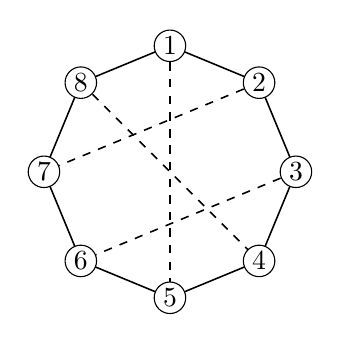
\begin{tikzpicture}[scale=0.4]


\draw [dashed] [black, line width=0.2mm] plot [smooth, tension=0] coordinates {(0,4) (0,-4)};
\draw [dashed] [black, line width=0.2mm] plot [smooth, tension=0] coordinates {(2.83,2.83) (-4,0)};
\draw [dashed] [black, line width=0.2mm] plot [smooth, tension=0] coordinates {(4,0) (-2.83,-2.83)};
\draw [dashed] [black, line width=0.2mm] plot [smooth, tension=0] coordinates {(-2.83,2.83) (2.83,-2.83)};

\draw [-] [black, line width=0.2mm] plot [smooth, tension=0] coordinates {(0,4) (2.83,2.83)};

\draw [-] [black, line width=0.2mm] plot [smooth, tension=0] coordinates {(4,0) (2.83,2.83)};


\draw [-] [black, line width=0.2mm] plot [smooth, tension=0] coordinates {(4,0) (2.83,-2.83)};

\draw [-] [black, line width=0.2mm] plot [smooth, tension=0] coordinates {(0,-4) (2.83,-2.83)};

\draw [-] [black, line width=0.2mm] plot [smooth, tension=0] coordinates {(0,-4) (-2.83,-2.83)};

\draw [-] [black, line width=0.2mm] plot [smooth, tension=0] coordinates {(-4,0) (-2.83,-2.83)};

\draw [-] [black, line width=0.2mm] plot [smooth, tension=0] coordinates {(-4,0) (-2.83,2.83)};

\draw [-] [black, line width=0.2mm] plot [smooth, tension=0] coordinates {(0,4) (-2.83,2.83)};


\draw[black,fill=white] (0,4) ellipse (0.5 cm  and 0.5 cm);
\draw[black,fill=white] (4,0) ellipse (0.5 cm  and 0.5 cm);
\draw[black,fill=white] (0,-4) ellipse (0.5 cm  and 0.5 cm);
\draw[black,fill=white] (-4,0) ellipse (0.5 cm  and 0.5 cm);
\draw[black,fill=white] (2.83,2.83) ellipse (0.5 cm  and 0.5 cm);
\draw[black,fill=white] (-2.83,-2.83) ellipse (0.5 cm  and 0.5 cm);
\draw[black,fill=white] (2.83,-2.83) ellipse (0.5 cm  and 0.5 cm);
\draw[black,fill=white] (-2.83,2.83) ellipse (0.5 cm  and 0.5 cm);

\node (1) at (0,4) {{1}};
\node (2) at (2.83,2.83) {{2}};
\node (3) at (4,0) {{3}};
\node (4) at (2.83,-2.83) {{4}};
\node (5) at (0,-4) {{5}};
\node (6) at (-2.83,-2.83) {{6}};
\node (7) at (-4,0) {{7}};
\node (8) at (-2.83,2.83) {{8}};
\end{tikzpicture}
\caption{A Carr-Vempala point with 8 vertices on its cycle. Solid lines are edges with value strictly between $0$ and $1$. Dashed edges represent paths where each edge on the path has $x_e =1$. There can be an arbitrary number of degree-$2$ vertices on the dashed paths.}
\label{fig:CVpoint}
\end{figure}

\begin{figure}[h!]
	\centering
	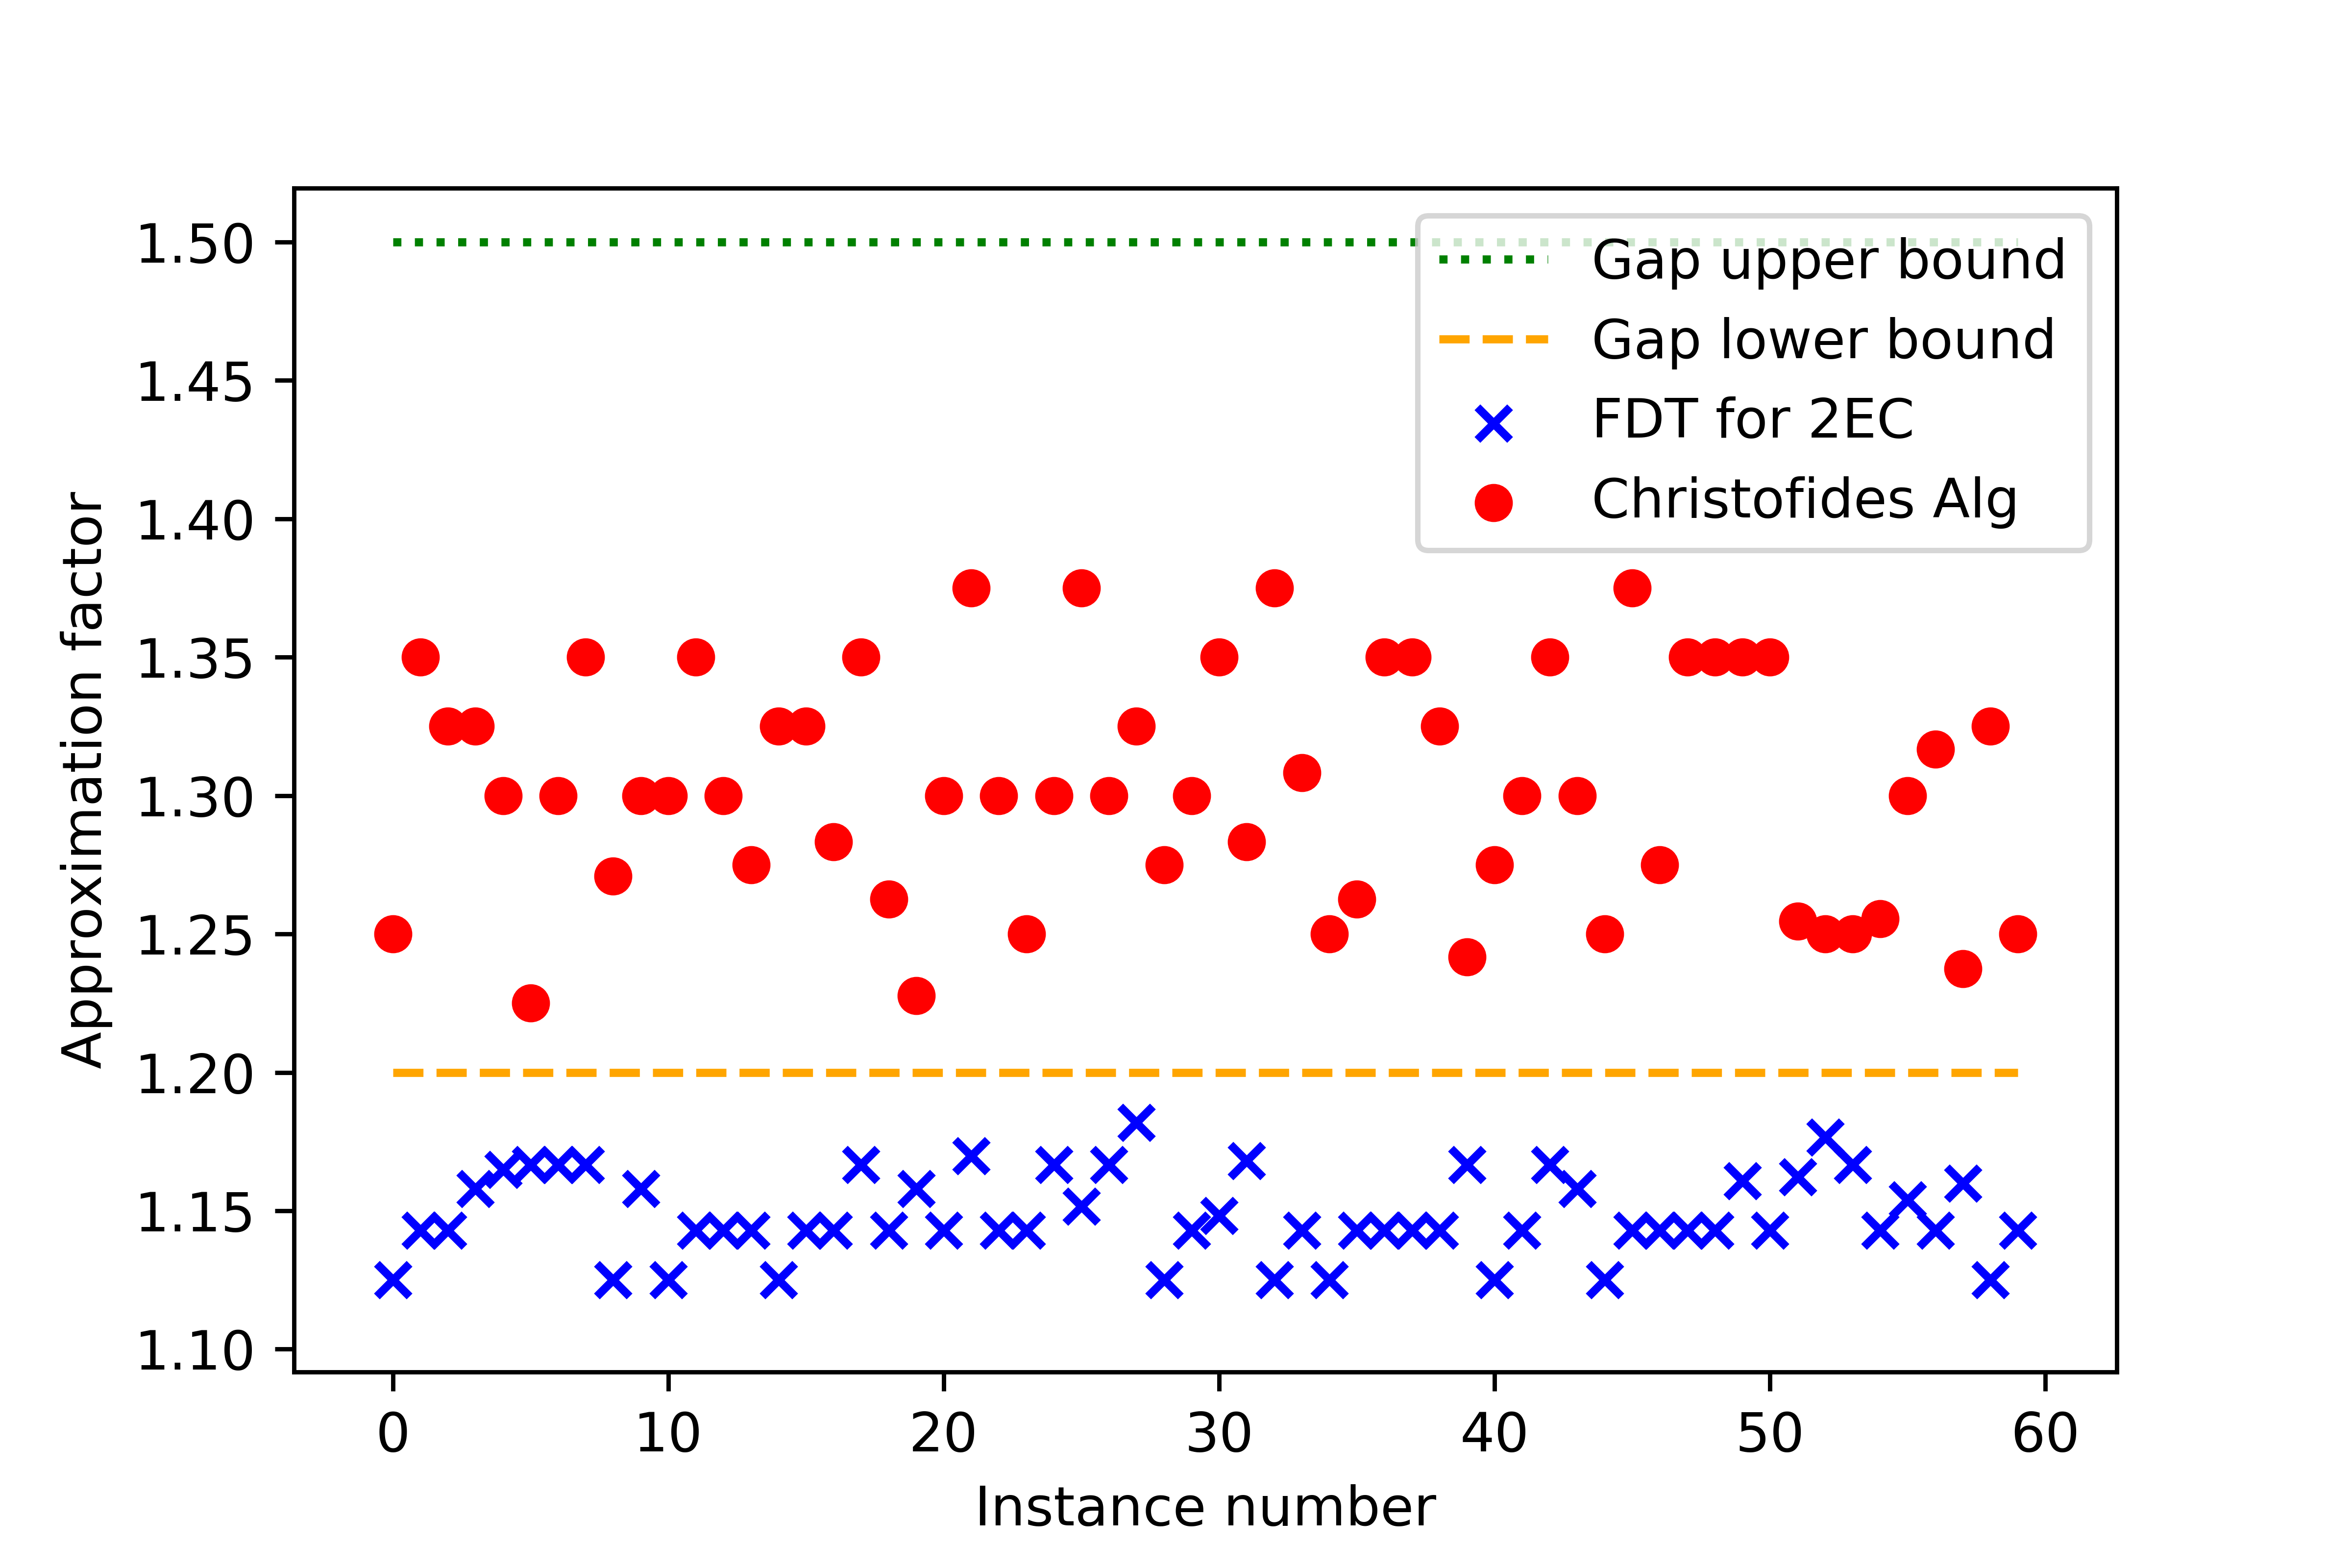
\includegraphics[width=9cm,scale=1.4]{christofides-vs-fdt.png}
	\caption{Polyhedral version of Christofides' algorithm vs FDT on all Carr-Vempala points that have 10 vertices on the single cycle formed by fractional edges.}
	\label{fdtvschris}
\end{figure}
\paragraph{FDT for 2EC on Carr-Vempala points.}
We ran FDT for 2EC on 963 fractional extreme points of $\subtour(G)$. We enumerated all (fractional) Carr-Vempala points with $10$ and $12$ vertices. Table \ref{table2EC} shows that again FDT found solutions better than the integrality-gap lower bound for most instances. 
\begin{table}[h!]
	\begin{small}
		\centering
		\begin{tabular}{c c c c c}
			\hline
			& $C\in [1.08,1.11]\;$ & $\;C\in (1.11,1.14]\;$ &
			$\;C\in (1.14,1.17]$ &\; $C\in (1.17,1.2]\;$ \\ \hline
			2EC & $79$ & $201$ & $605$ & $78$ \\ \hline\\
		\end{tabular}	\caption{FDT for $\2ec$ implemented applied to all Carr-Vempala with 10 or 12 vertices. A Carr-Vempala point with $k$ vertices has $\frac{3k}{2}$ edges. Thus, the upper bound provided by Theorem \ref{FDT2EC} is $g(\2ec)^{3k/2}$. The lower bound on $g(\2ec)$ is $\frac{6}{5}$.}
		\label{table2EC}
	\end{small}
\end{table}


